\chapter{My work}
\label{cha:main}
\textit{Schema of the final solution, explanation of the flow and how it concretely works. Then, focus on three key components.}

\begin{figure}[H]
    \centering
    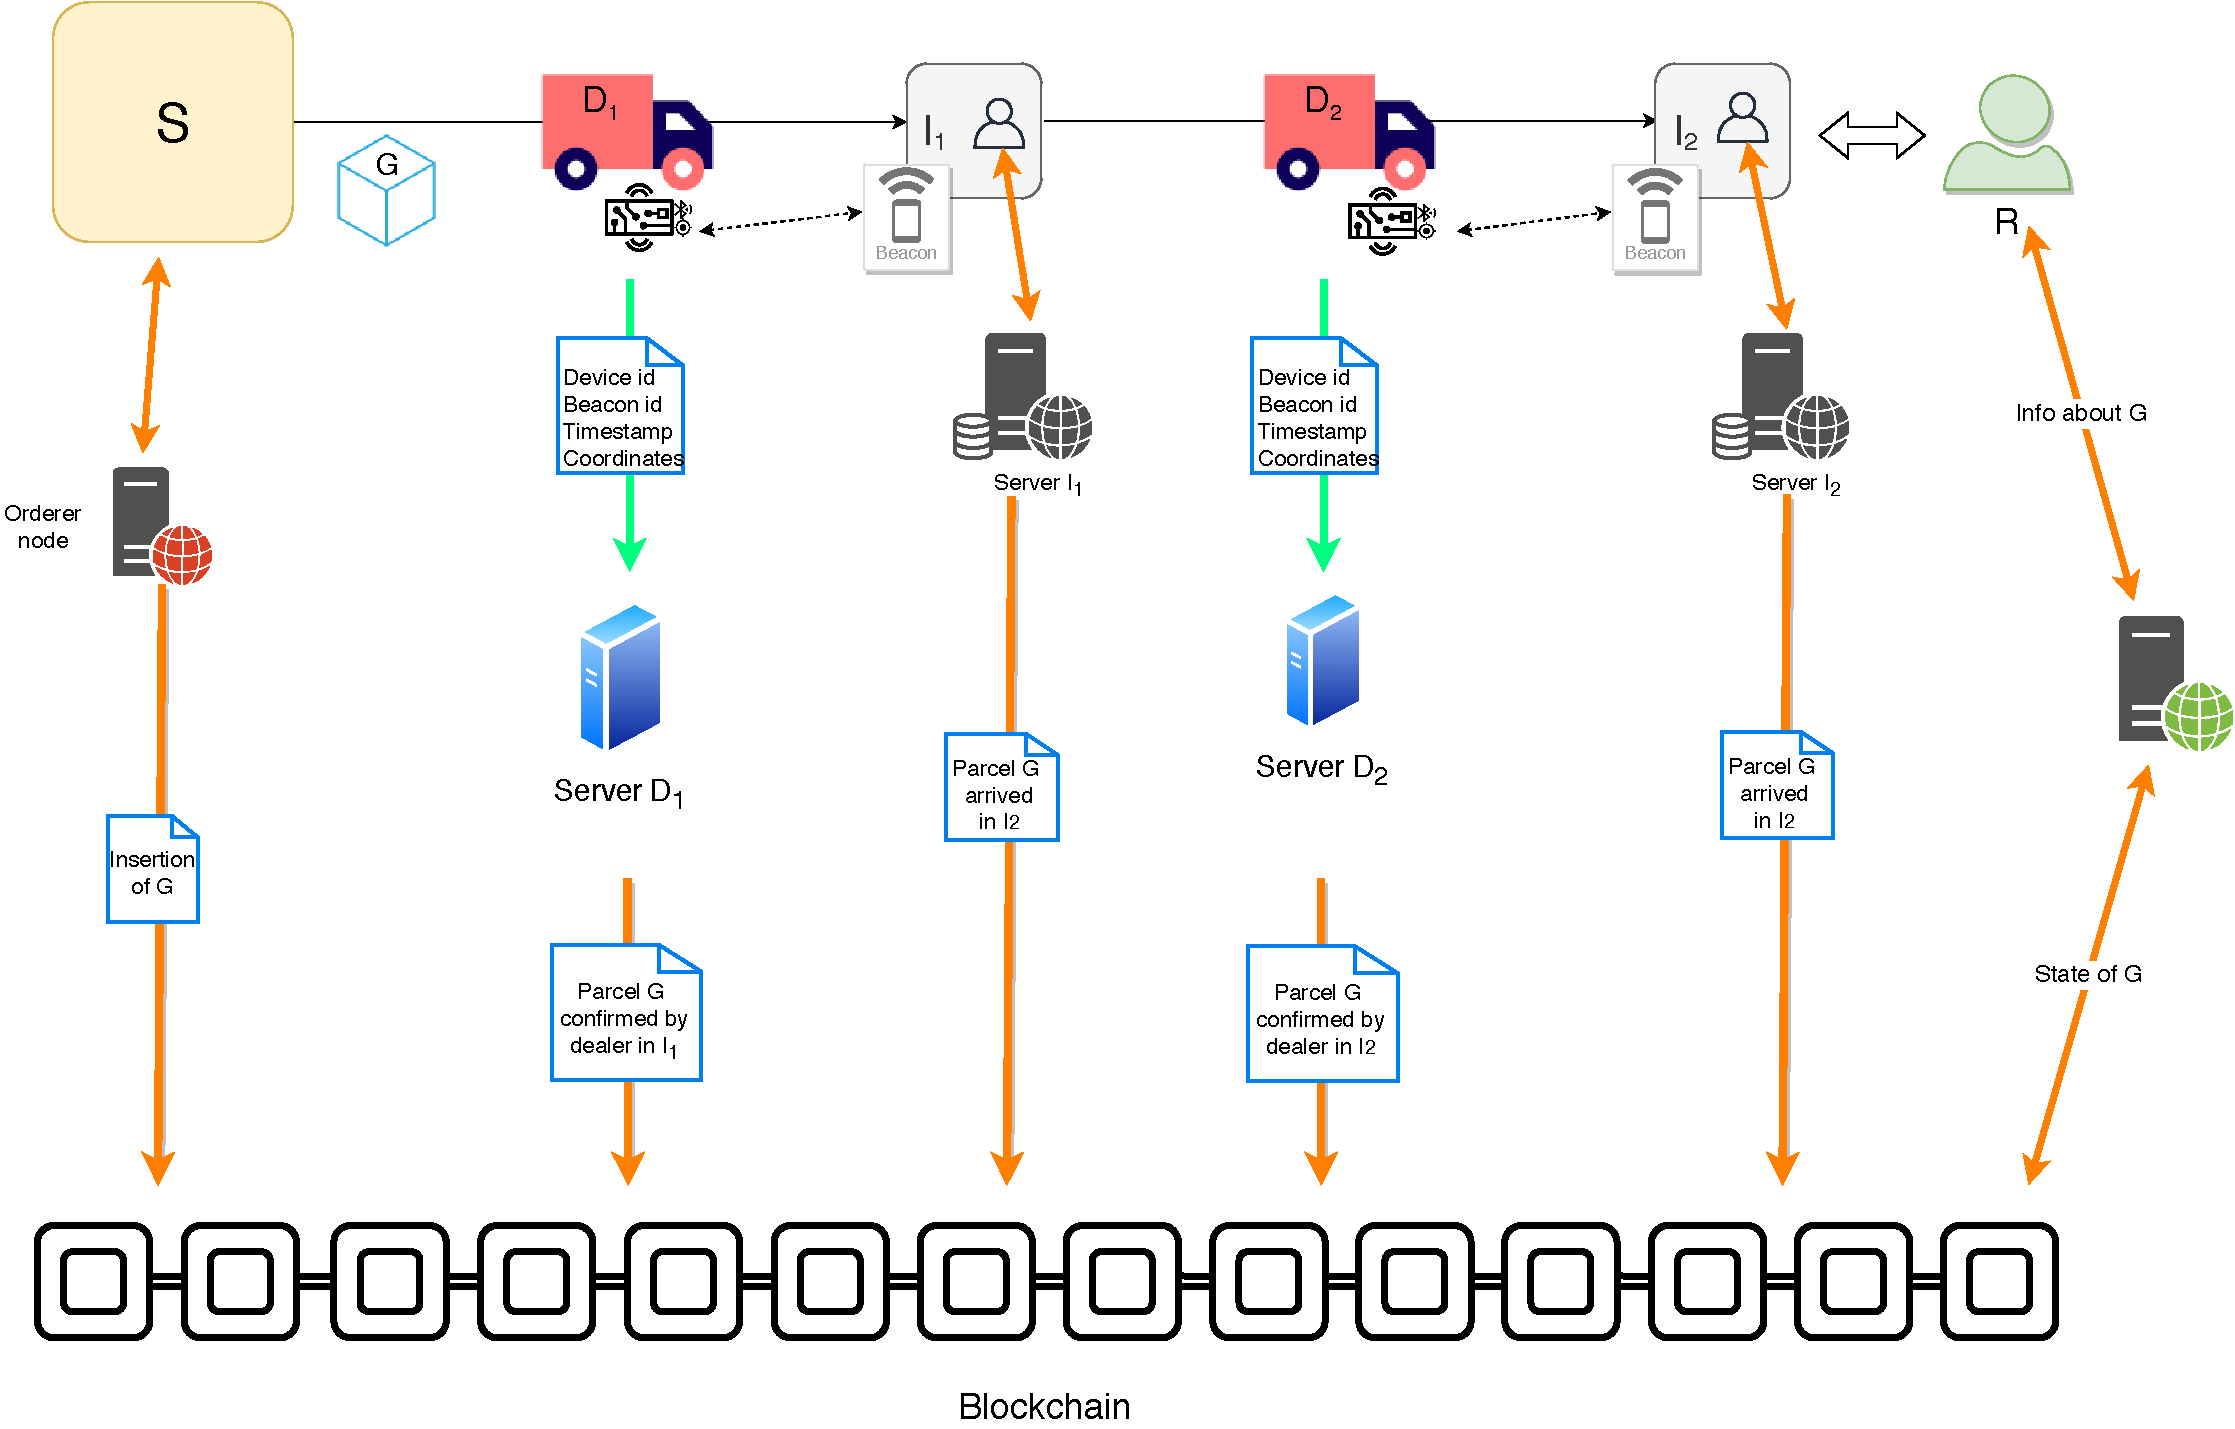
\includegraphics[scale=0.45]{figures/solution.pdf}
    \caption{The schema of the discussed solution}
    \label{fig:solution}
\end{figure}

Figure \ref{fig:solution} illustrates the solution that I have elaborated during my internship. Let us explain its characteristics, by first analyzing the overall flow and then concentrating in each step.

The notation used in the schema is the same as the one introduced in chapter \ref{cha:background}: from left to right, we notice the sender \textit{S}, the good \textit{G}, two dealers $D_1$ and $D_2$, two intermediate points $I_1$ and $I_2$ (each one with a responsible person at work) and finally the receiver $R$. Obviously, this scenario is just a possible combination of entities and the solution is not fixed to this one.

The following is an abstract description of the various actions that are part of the model. For this moment we are ignoring some specific details (e.g. the protocols used for interactions, the format of the packets etc.), that will be properly explained together with the singular components.

$S$ starts the process by inserting into the system the information related to $G$. They have a dedicated server to provide the requested data. In particular, they need to declare the intermediate points and the dealers. This data will be stored in the blockchain as a new ``asset'', something similar to the coins in crypto-currencies. 

Then, the delivery is ready to start. $D_i$ (the procedure holds for both $D_1$ and $D_2$) carries an IoT device tracking its location and searching for other BLE devices nearby. On the other side, the intermediate stop has a beacon, constantly advertising its UUID (Universally Unique IDentifier). The protocol for the exchange is the following: 
\begin{itemize}
    \item The dealer arrives at the destination, the tracker detects the stop and sends to a server a packet containing the beacons' identifiers found;
    \item The server controls if one of the identifiers corresponds to the one owned by the intermediary and, if so, sends a confirmation to the blockchain;
    \item The person in control of $I_j$ collects $G$ and sends a confirmation, using a web interface, to a separate web server.
\end{itemize}

The model as it is so far cannot be deceived by the dealer, as they have no control over the device; however, it is vulnerable to an attack from a malicious actor controlling $I$. They can, in fact, collect $G$ and not inform the system about the exchange. As a result, we have lost track of who has the good. To solve this, there is the need for a protocol on the ``human'' side. Not complicated, but essential: the dealer has to make sure that who receives $G$ really sends their confirmation to the server. 

The final recipient, at any time, can access an interface that, by consulting the status of G on the blockchain, informs him about the progress of the delivery. They can check which exchanges happened and whether they succeeded. In case of problems it is immediate to find the responsible. Assuming that the protocol has been fully respected, if $G$ is only confirmed by the dealer it means that it is still in their hands; to the contrary, if only the intermediary confirmed the good an error must have occurred, because there is no proof that the dealer really arrived at that place.

After this brief analysis there are a lot of unknown elements: how the devices work, how the communications take place, how the data is actually saved. In the next sections we will discuss these aspects, dividing the project into the three main branches that constitute it.


\section{Tracking}
\label{sec:tracking}
%Introduction to what kind of tracking is needed, what we expect from the devices. Brief explanation of the state of the art of communication technologies (LoRa, SigFox, LTE, Wi-Fi, BLE, ...) and geolocalization.

The first part that we analyze is the tracking. Our solution needs devices that support geolocalization, bluetooth and can connect to the Internet to send messages. Clearly these are just the basic requirements, additional features can be useful in future developments. Another important aspect is the battery, since these devices cannot ensure long autonomy if frequently active. 

First, we will give a brief description of the modern technologies for the communications of IoT devices, then we will dive into the market to analyze the various options.

\subsection{Communication technologies}
\label{sec:track_comm}
\textit{A brief analysis over the existing tracking technologies}

The state-of-the-art of these networks is very wide and presents several alternatives, each of them with advantages and disadvantages. They can be divided by many parameters, since many variables need to be taken into account when modelling the architecture of an IoT project. Our use case requires a standard able to guarantee the delivery of packets at arbitrary distance, consuming as little battery as possible. These requirements drive us to a new wireless communication techonology: LPWAN (Low Power Wide Area Network).

LPWAN is increasingly becoming popular thanks to its low-power, long-range and low-cost communication properties. It is particularly suitable for IoT applications that only need to transmit small amounts of data in long range and for its specifications it is preferable to traditional cellular options (such as 4G and LTE networks).

Many LPWAN technologies have been developed in both the licensed and unlicensed frequency bands. LoRa, Sigfox and NB-IoT are today the leading ones, with many technical differences \cite{LPWAN_study}.

\subsubsection{LoRa}
LoRa (Long Range) is a patented digital wireless data communication technology that was first developed by Cycleo - a French start-up - and then acquired by Semtech (USA). Its ecosystem can be divided in two parts, LoRa and LoRaWAN: the latter is the standard protocol for WAN communications and the former is used as a wide area network technology. In other words, LoRa is the physical layer and LoRaWAN is the MAC and application layer of the stack.

LoRaWAN provides various classes of end devices to address different requirements. It ensures a better battery life compared to the other LPWAN technologies, but this also implies lower data rates and longer latency. To connect to the Internet, LoRa requires a gateway. The infrastructure is the following: end devices communicate with one or more LoRa gateways, which then forward messages to a cloud, a network server or to another gateway. On the contrary, when a message is sent to a device, the network chooses the best gateway.

One important aspect of LoRaWAN is determined by the so-called duty-cycle: defined as the maximum percentage of time during which an end-device can occupy a channel, is a key constraint for networks operating in unlicensed bands. Thus, each device has a threshold limiting the overall transmission time. However, the amount that a device will need is unknown, since it depends on the distance between the end point and the nearest gateway. The farther the gateway, the longer it will take to deliver a message. As a result, the total amount of messages sent is unknown and totally unpredictable considering our use case, in which we cannot make assumptions on the distribution of the gateways (w.r.t. the location of the tracker).

To sum up: LoRaWAN is not proprietary and offers quite a good amount of flexibility, but it has some problems of coverage and infrastructure that does not make it the best choice.

\subsubsection{Sigfox}
Sigfox is a patented technology that was developed in 2010 by the start-up SigFox. It is an LPWAN network operator that uses a wide-reaching signal called ``ultra narrow-band''. This system presents a significant link asymmetry: a downlink communication, i.e., data from the base stations to the end devices can only occur following an uplink communication and in every case the number of messages is limited to four per day. On the uplink, instead, the amount of packets sent cannot be more than 140 per day, with a maximum payload length of 12 bytes. Clearly, acknowledgements cannot be supported and consequently the reliability is ensured using time and frequency diversity as well as transmission duplication.

Sigfox is an interesting technology, but it has similar limitations to LoRaWAN as regards the messages that can be sent: in fact, they were included by the designers for the same reasons.

\subsubsection{NB-IoT}
NB-IoT is a radio technology standard developed by 3GPP (3rd Generation Partnership Project) to enable a wide range of cellular devices and services. It is based on the LTE protocol, therefore guaranteeing the high performance level associated with cellular connections, but at the cost of more complexity and greater power consumption. While other infrastructures have gateways that aggregate sensor data, which then communicate with the primary server, with NB-IoT sensor data is sent directly to it. For this reason it is being touted as the potentially less expensive option.

LTE-M is another LPWAN radio technology standard based on LTE. However, we did not take it into consideration because there is a lack of coverage and support from operators in Italy.

We can conclude that, for our use case, the NB-IoT is the best alternative: despite the higher battery usage, it offers a solid and unrestricted network that can be used without creating a particular infrastructure or having to limit the number of messages.


\subsection{The market}
\textit{The study and testing of the alternatives available, maybe a table summarizing the characteristics of each device (type of communication supported, battery, personalization of firmware, cost).}

The market of the IoT is constantly growing. There are numerous applications for these devices, both indoors and outdoors, with a variety of different requirements. For this reason almost every company offers more than one solution, to best meet the needs of the buyer. We proceed now with the analysis of the most relevant trackers, outlining the specifications of each of them.



\subsection{Pycom}
\label{sec:track_choice}
\textit{Why we decided to choose that device: possibility to fully program the firmware, connectivity...}

\subsection{Firmware}
\label{sec:track_firmware}
\textit{Life cycle of the device (maybe with a flow chart). Some snippets?}

\section{Decentralized architecture}
\label{sec:arch}
\textit{Requirements of the architectures, same as \ref{sec:tracking} (what we expect etc).}

\subsection{Decentralization alternatives}
\label{sec:alternatives}
\textit{Distributed databases, how they reach consensus, permissioned vs permissionless, blockchain based frameworks.}

\subsection{HyperLedger}
\label{sec:hyperledger}
\textit{Why (free and open source, easy to use, easy to install and deploy - mentioning Docker), description of what it is and how it works. Schema with their grammar of our network.}


\section{Interfaces/Servers}
\textit{Small section with a bit of reference about the webapps and how they work, what should be allowed. Some snippets can be useful here, explaining how we make use of hyperledger APIs. A little paragraph describing what MQTT is and why we decided to use it.}

